\documentclass[11pt, oneside]{article}   	% use "amsart" instead of "article" for AMSLaTeX format
\usepackage{geometry}                		% See geometry.pdf to learn the layout options. There are lots.
\geometry{letterpaper}                   		% ... or a4paper or a5paper or ... 
%\geometry{landscape}                		% Activate for for rotated page geometry
%\usepackage[parfill]{parskip}    		% Activate to begin paragraphs with an empty line rather than an indent
\usepackage{graphicx}				% Use pdf, png, jpg, or eps� with pdflatex; use eps in DVI mode
								% TeX will automatically convert eps --> pdf in pdflatex		
\usepackage{amssymb}
\usepackage{amsmath}
\usepackage{parskip}
\usepackage{color}
\usepackage{hyperref}

\title{Quick Double Integrals}
%\author{The Author}
%\section{}
%\subsection*{}
\date{}							% Activate to display a given date or no date

\graphicspath{{/Users/telliott_admin/Dropbox/Tex/png/}}
% \begin{center} 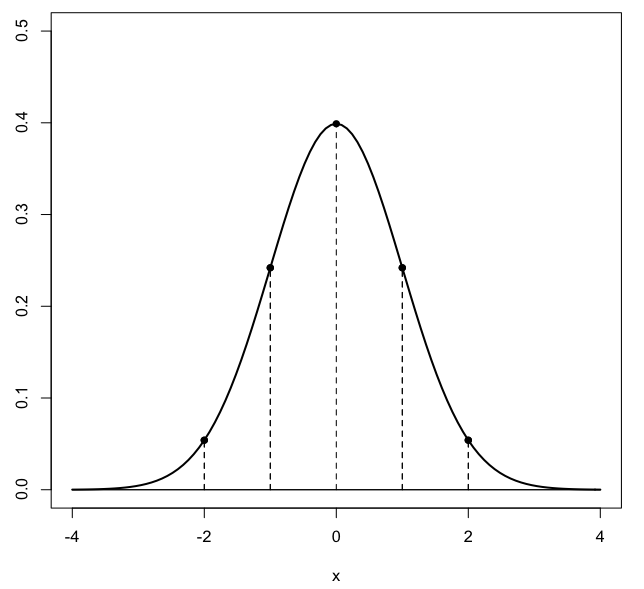
\includegraphics [scale=0.4] {gauss3.png} \end{center}
\begin{document}
\maketitle
\Large
In this short write-up I want to take a very quick look at double integrals.  The basic principle of calculus of several variables is that we look at the effect of small changes in \emph{one variable at a time}.  So we write
\[ df = \frac{\partial f}{\partial x} dx + \frac{\partial f}{\partial y} dy \]
where, for example, $\partial f/\partial x$ is the derivative of $f$ with respect to $x$, treating $y$ as a constant.

For integration, consider a rectangle where $x$ varies between $0 \rightarrow 2$, while $y = 0 \rightarrow 3$.  To compute the area of this rectangle, we write
\[ A = \int_{x=0}^{2} \int_{y=0}^{3} \ dy \ dx \]
There is no $f(x,y)$ inside the integral sign (except implicitly $f(x,y)=1$), and the result will be the area.  In the same way $\int dx = x_f - x_i$, the length of $x$.

To evaluate the integral, look at the part inside, the inner integral
\[ \int_{y=0}^{3} \ dy \]
We need a function whose derivative is $dy$, holding $x$ constant.  In this case, that's just $y$, evaluated between the limits.  We obtain
\[ \int_{y=0}^{3} \ dy = y \ \bigg |_0^3 = 3 \]
So we proceed to evaluate the outer integral
\[ A = \int_{x=0}^{2} 3 \ dx = 3 \int_{x=0}^{2} \ dx = 3 \times 2 = 6 \]

\subsection*{something more ambitious}
Now consider a circle.  We're going to integrate the function $f(x,y) =1$ over a circle of radius $R$.  For simplicity, we do only the first quadrant, and multiply at the end by $4$.
\[ A = \int_{x=0}^R \int_{y=0}^{\sqrt{R^2 - x^2}} \ dy \ dx \]
Since $y$ changes as a function of $x$, we need to account for that.  That's why we have the upper limit on $y$.  The inner integral is easy
\[ \int_{y=0}^{\sqrt{R^2 - x^2}} \ dy = \sqrt{R^2 - x^2} \]
But now the outer integral is
\[ A = \int_{x=0}^R \sqrt{R^2 - x^2} \ dx \]
This presents a bit of a problem because we don't have the derivative for what's inside the square root.  We continue anyway, with a trig substitution.
\[ x = R \sin \theta \]
\[ dx = R \cos \theta \ d \theta \]
\[ \sqrt{R^2 - x^2} = R \cos \theta \]
So the integral is
\[ \int R^2 \cos^2 \theta \ d \theta \]
I've done this before.  The answer is
\[ = R^2 \ \frac{1}{2} ( \theta + \sin \theta \cos \theta) \]
The really tricky part is the limits.  We could switch back to $x$ or we can recognize that when $x=R$, $\sin \theta = 1$ and when $x=0$, $\sin \theta = 0$ so we evaluate between $\theta = 0 \rightarrow \pi/2$.  That makes $\sin \theta \cos \theta$ go away.  The result is just
\[ = R^2 \ \frac{1}{2} (\frac{\pi}{2} ) \]
Multiply by $4$ to obtain $\pi R^2$.

\subsection*{an easier way}
There is another approach, which is the reason for this particular write-up.  The "area element" in 2D using polar coordinates is
\[ dA = r \ dr \ d \theta \]
\begin{center} 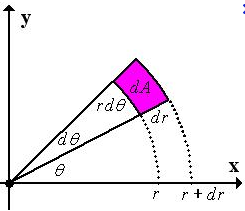
\includegraphics [scale=0.75] {polararea.png} \end{center}
The figure shows a rationale for this.  $\theta$ or $d \theta$ is not a length, $r \ d \theta$ is a length.  What we're saying is that the area element in the plane is
\[ dA = dy \ dx = r \ dr \ d \theta \]
and for any particular region, we can pick the one that's easier.  Clearly, for a circle, the second way is easier.  We set up the integral
\[ A = \int_{\theta = 0}^{2 \pi} \int_{r=0}^{R} r \ dr \ d \theta \]
The inner integral is
\[ \int_{r=0}^{R} r \ dr = \frac{r^2}{2} \ \bigg |_{r=0}^{R}  = \frac{R^2}{2} \]
The outer integral is
\[ A = \int_{\theta = 0}^{2 \pi} \frac{R^2}{2} \ d \theta = \frac{R^2}{2} \ 2 \pi = \pi R^2  \]

\subsection*{application}
We can apply what we've learned to the following problem.  In the Gaussian distribution and also in the physics of molecular velocities we run into an integral like
\[ I = \int_{-\infty}^{\infty} e^{-x^2} \ dx \]
There is a great solution to this.  Write
\[ I^2 = \int_{-\infty}^{\infty} e^{-x^2} \ dx \int_{-\infty}^{\infty} e^{-y^2} \ dy \]
\[ = \int_{-\infty}^{\infty} \int_{-\infty}^{\infty}  e^{-(x^2 + y^2)} \ dx \ dy \]
But we can change this to polar coordinates
\[ = \int_0^{2 \pi} \int_{0}^{\infty} e^{-r^2} \ r \ dr \ d \theta \]
The inner integral is just
\[ \int_{0}^{\infty} e^{-r^2} \ r \ dr = -\frac{1}{2}e^{-r^2} \ \bigg |_0^{\infty} = \frac{1}{2}  \]
So then we have 
\[ I^2 = \int_0^{2 \pi} \frac{1}{2} \ d \theta = \pi  \]
To put this another way
\[ I = \sqrt{\pi} \]
\[  I = \int_{-\infty}^{\infty} e^{-x^2} \ dx = \sqrt{\pi} \]


\end{document}  